\chapter{Testing}
\label{chap:testing} 

Dieses Kapitel beschreibt wie wir unseren Bot und dessen Komponenten getestet haben. Das Testen beanspruchte ein grosser Teil unserer aufgewendeten Zeit. Die nachfolgenden Methoden zeigen auf wie wir versuchten m�glichst effizient zu testen, so dass uns mehr Zeit f�r das implementieren von Modulen blieb. Es stellte sich heraus, dass das Implementieren und Testen von neuem Code in UnitTests anstatt direkt im Bot, zeitsparender war und weniger M�he bereitete Fehler zu finden. 

\section{Unit Tests}
\label{sec:testCenter.UniTests}

Danke dem modularen Aufbau des Java-Codes war es uns m�glich einzelne Module zu testen. F�r unsere UnitTests verwendeten wir die JUnit 4 Library. So hat jedes Java Project ein UnitTest-Package. Der Code im Java Project wird durch diverse Testklassen im UnitTest-Package auf die Richtigkeit gepr�ft. Die hat den Vorteil, das wir funktionierende Module in den Bot einbauen konnten, und nicht erst nach dem Einbau nach Fehlern suchen mussten.\\
Um das Modul CombatPositioning (siehe im Code unter Startegy.tactics.combat) zu realisieren haben wir sogar 'Test Driven Development' eingesetzt. Dass heisst wir haben zuerst den Test mit Ausgangslage, Aufruf von CombatPositioning, und das erwartete Resultat geschrieben. Danach wurde solange an CombatPositioning programmiert, bis das erwartete Testresultat eintraf.

\section{Visuelle Tests}
\label{sec:testCenter.VisuelleTests}

In Form eines UnitTest haben wir auch unsere visuellen Tests geschrieben. Durch eine visuelle �berpr�fung des Resulats ist meistens, vorallem bei der Pfadsuche, einfacher zu kontrollieren. Anstatt aber mit der JUnit Methode \textit{assertEquals()} das Resultat zu pr�fen haben die visuellen Test ein HTML-File als Output. In das HTML-File wird die Karte in Tabellenform gespeichert. In jeder Zelle der Tabelle k�nnen Objekte (Einheiten, H�gel, Wegpunkte, etc.) mittels farbige Punkte dargestellt werden. Diese Funktionalit�ten bietet die extra geschriebene Klasse MapOutput. Nachfolgend ist ein HTML-File abbgebildet mit welchem wir die Korrektheit des Clustering und des HPA* Algorithmus visuelle �berpr�ft haben. 

TODO mapoutput01?
%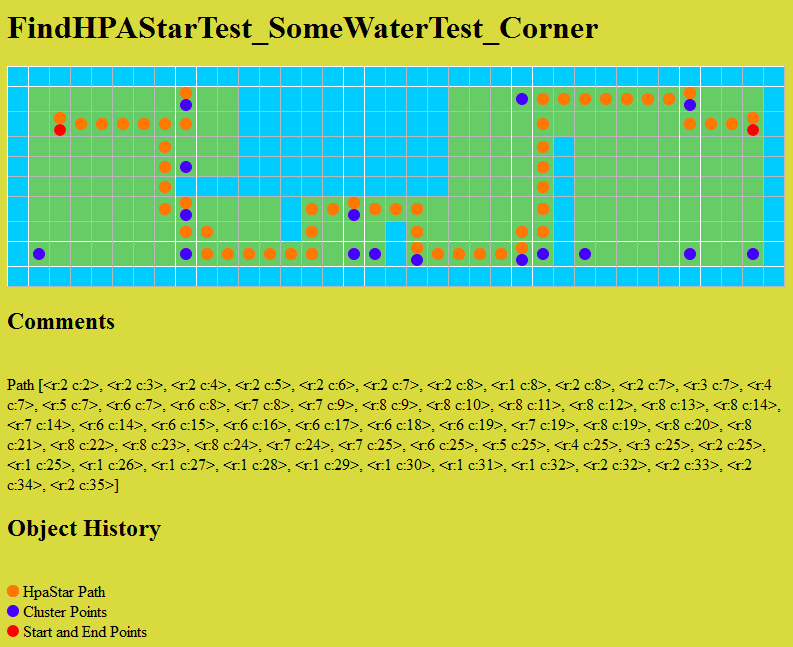
\includegraphics[height=50mm]{91_bilder/mapoutput01}
%\caption{HTML-File zur visuellen �berpr�fung von HPA*}
%\label{fig:mapoutput01}
%\end{figure}